% ============================================================
% 讲义 — 人教版七年级下册 · 第7章 平面直角坐标系
% 编译命令：xelatex -interaction=nonstopmode 第7章_平面直角坐标系.tex
% ============================================================
\documentclass[12pt, a4paper]{ctexart}
\usepackage[margin=2.2cm]{geometry}
\usepackage{amsmath, amssymb}
\usepackage{enumitem}
\usepackage{tcolorbox}
\usepackage{booktabs}
\usepackage{array}
\usepackage{fancyhdr}
\usepackage{xcolor}
\usepackage{tikz}
\usepackage{hyperref}
\usepackage{graphicx}
\usepackage{multirow}
\usepackage{pgfplots}
\pgfplotsset{compat=1.18}

% 颜色定义
\definecolor{mainblue}{RGB}{41, 98, 168}
\definecolor{lightblue}{RGB}{230, 240, 255}
\definecolor{tipgreen}{RGB}{34, 139, 87}
\definecolor{lightgreen}{RGB}{235, 250, 240}
\definecolor{warnred}{RGB}{200, 50, 50}
\definecolor{lightred}{RGB}{255, 240, 240}
\definecolor{examorange}{RGB}{210, 120, 20}
\definecolor{lightorange}{RGB}{255, 248, 235}
\definecolor{apppurple}{RGB}{120, 60, 170}
\definecolor{lightpurple}{RGB}{245, 238, 255}

% 页眉页脚
\pagestyle{fancy}
\fancyhf{}
\fancyhead[L]{\small\textcolor{mainblue}{\textbf{人教版七年级下册 · 第7章 平面直角坐标系}}}
\fancyhead[R]{\small\textcolor{mainblue}{家教讲义}}
\fancyfoot[C]{\small —\ \thepage\ —}
\renewcommand{\headrulewidth}{0.6pt}
\renewcommand{\headrule}{\hbox to\headwidth{\color{mainblue}\leaders\hrule height \headrulewidth\hfill}}
\renewcommand{\footrulewidth}{0pt}

% tcolorbox 样式
\newtcolorbox{knowledgebox}[1][]{%
  colback=lightblue, colframe=mainblue,
  fonttitle=\bfseries\large, title=#1,
  arc=3mm, boxrule=0.8pt,
  left=8pt, right=8pt, top=6pt, bottom=6pt
}

\newtcolorbox{tipbox}[1][]{%
  colback=lightgreen, colframe=tipgreen,
  fonttitle=\bfseries, title=#1,
  arc=2mm, boxrule=0.6pt,
  left=6pt, right=6pt, top=4pt, bottom=4pt
}

\newtcolorbox{warnbox}[1][]{%
  colback=lightred, colframe=warnred,
  fonttitle=\bfseries, title=#1,
  arc=2mm, boxrule=0.6pt,
  left=6pt, right=6pt, top=4pt, bottom=4pt
}

\newtcolorbox{examplebox}[1][]{%
  colback=lightorange, colframe=examorange,
  fonttitle=\bfseries, title=#1,
  arc=3mm, boxrule=0.8pt,
  left=8pt, right=8pt, top=6pt, bottom=6pt
}

\newtcolorbox{appbox}[1][]{%
  colback=lightpurple, colframe=apppurple,
  fonttitle=\bfseries, title=#1,
  arc=3mm, boxrule=0.8pt,
  left=8pt, right=8pt, top=6pt, bottom=6pt
}

\setCJKmainfont{Hiragino Sans GB}
\setCJKsansfont{Heiti SC}

% 填空命令
\newcommand{\blank}[1]{\underline{\hspace{#1}}}

\begin{document}

% ============ 标题页 ============
\begin{center}
{\Huge\bfseries\textcolor{mainblue}{第7章\quad 平面直角坐标系}}\\[12pt]
{\Large\textcolor{gray}{家\quad 教\quad 讲\quad 义}}\\[8pt]
\rule{0.6\textwidth}{1pt}\\[8pt]
{\normalsize 适用：人教版\quad 七年级下册\quad |\quad 课时：4课时}
\end{center}
\vspace{10pt}

% ==============================================================
% 第一部分：知识点讲解
% ==============================================================
\section*{\textcolor{mainblue}{一、知识点讲解}}

% ---- 7.1 有序数对 ----
\subsection*{7.1\quad 有序数对}

\begin{knowledgebox}[有序数对的概念]
我们把有顺序的两个数 $a$ 与 $b$ 组成的数对，叫做\textbf{有序数对}，记作 $(a, b)$。

\medskip
\textbf{关键要点：}
\begin{itemize}[leftmargin=1.5em]
  \item "有序"意味着顺序不能调换：$(a, b) \neq (b, a)$（除非 $a = b$）。
  \item 有序数对可以用来确定平面内点的位置。
  \item 例如：电影票上的"第3排第5座"可以用 $(3, 5)$ 表示。
\end{itemize}
\end{knowledgebox}

\begin{warnbox}[易错提醒]
$(2, 3)$ 和 $(3, 2)$ 是两个\textbf{不同}的有序数对，对应平面内\textbf{不同}的位置。书写时一定要注意顺序！
\end{warnbox}

% ---- 7.2 平面直角坐标系 ----
\subsection*{7.2\quad 平面直角坐标系}

\begin{knowledgebox}[平面直角坐标系的构成]
在平面内画两条\textbf{互相垂直}、\textbf{原点重合}的数轴，就组成了\textbf{平面直角坐标系}。

\medskip
\textbf{组成要素：}
\begin{itemize}[leftmargin=1.5em]
  \item \textbf{横轴（$x$ 轴）}：水平方向的数轴，向右为正方向。
  \item \textbf{纵轴（$y$ 轴）}：竖直方向的数轴，向上为正方向。
  \item \textbf{原点 $O$}：两条数轴的交点，坐标为 $(0, 0)$。
  \item 两条坐标轴将平面分成四个部分，称为\textbf{四个象限}。
\end{itemize}

\medskip
\textbf{四个象限（逆时针编号）：}

\begin{center}
\begin{tikzpicture}[scale=0.8]
  % 画坐标轴
  \draw[->, thick, mainblue] (-4.5,0) -- (4.5,0) node[right]{$x$};
  \draw[->, thick, mainblue] (0,-3.5) -- (0,3.5) node[above]{$y$};
  \node[mainblue] at (0,0) [below left]{$O$};
  % 象限标注
  \node[mainblue, font=\large\bfseries] at ( 2.5, 2) {一};
  \node[mainblue, font=\large\bfseries] at (-2.5, 2) {二};
  \node[mainblue, font=\large\bfseries] at (-2.5,-2) {三};
  \node[mainblue, font=\large\bfseries] at ( 2.5,-2) {四};
  % 刻度
  \foreach \x in {-4,-3,-2,-1,1,2,3,4}
    \draw[mainblue] (\x,0.15) -- (\x,-0.15);
  \foreach \y in {-3,-2,-1,1,2,3}
    \draw[mainblue] (0.15,\y) -- (-0.15,\y);
  \node[mainblue] at (1,0) [below right]{\small 1};
  \node[mainblue] at (0,1) [above left]{\small 1};
\end{tikzpicture}
\end{center}
\end{knowledgebox}

\begin{knowledgebox}[点的坐标]
对于平面内任意一点 $P$，过点 $P$ 分别向 $x$ 轴和 $y$ 轴作垂线，垂足在 $x$ 轴上对应的数为 $a$，在 $y$ 轴上对应的数为 $b$，则点 $P$ 的坐标为 $(a, b)$，其中 $a$ 叫做\textbf{横坐标}，$b$ 叫做\textbf{纵坐标}。
\end{knowledgebox}

% ---- 7.3 各象限及坐标轴上点的特征 ----
\subsection*{7.3\quad 各象限及坐标轴上点的坐标特征}

\begin{knowledgebox}[各象限内点的坐标符号]
\begin{center}
\renewcommand{\arraystretch}{1.4}
\begin{tabular}{|c|c|c|}
  \hline
  \textbf{象限} & \textbf{横坐标 $x$} & \textbf{纵坐标 $y$} \\
  \hline
  第一象限 & $+$ & $+$ \\
  \hline
  第二象限 & $-$ & $+$ \\
  \hline
  第三象限 & $-$ & $-$ \\
  \hline
  第四象限 & $+$ & $-$ \\
  \hline
\end{tabular}
\end{center}

\medskip
\textbf{记忆口诀：}一全正，二纵正，三全负，四横正。

\medskip
\textbf{坐标轴上点的特征：}
\begin{itemize}[leftmargin=1.5em]
  \item $x$ 轴上的点：纵坐标 $y = 0$，即 $(a, 0)$。
  \item $y$ 轴上的点：横坐标 $x = 0$，即 $(0, b)$。
  \item 原点：$(0, 0)$。
\end{itemize}

\medskip
\textbf{注意：}坐标轴上的点\textbf{不属于}任何象限！
\end{knowledgebox}

\begin{warnbox}[易错提醒]
\begin{itemize}[leftmargin=1.5em]
  \item 原点既在 $x$ 轴上，又在 $y$ 轴上，但它不属于任何象限。
  \item 判断点在哪个象限，只需看横、纵坐标的正负号，不要和数轴上的正负方向混淆。
  \item 第二象限的点横坐标为负、纵坐标为正，不要记反。
\end{itemize}
\end{warnbox}

% ---- 7.4 点到坐标轴的距离 ----
\subsection*{7.4\quad 点到坐标轴的距离}

\begin{knowledgebox}[点到坐标轴的距离]
设点 $P(a, b)$，则：
\begin{itemize}[leftmargin=1.5em]
  \item 点 $P$ 到 $x$ 轴的距离 $= |b|$（纵坐标的绝对值）。
  \item 点 $P$ 到 $y$ 轴的距离 $= |a|$（横坐标的绝对值）。
\end{itemize}
\end{knowledgebox}

\begin{tipbox}[规律总结]
点到 $x$ 轴的距离看\textbf{纵}坐标，点到 $y$ 轴的距离看\textbf{横}坐标。取绝对值即可，因为距离恒为非负数。
\end{tipbox}

% ---- 7.5 对称点的坐标关系 ----
\subsection*{7.5\quad 关于坐标轴和原点对称的点}

\begin{knowledgebox}[对称点的坐标关系]
设点 $P(a, b)$，则：

\begin{center}
\renewcommand{\arraystretch}{1.5}
\begin{tabular}{|c|c|}
  \hline
  \textbf{对称关系} & \textbf{对称点坐标} \\
  \hline
  关于 $x$ 轴对称 & $(a, -b)$ \quad 横同纵反 \\
  \hline
  关于 $y$ 轴对称 & $(-a, b)$ \quad 横反纵同 \\
  \hline
  关于原点对称 & $(-a, -b)$ \quad 横纵皆反 \\
  \hline
\end{tabular}
\end{center}

\medskip
\textbf{图示：关于原点对称}

\begin{center}
\begin{tikzpicture}[scale=0.9]
  \draw[->, thick, mainblue] (-4,0) -- (4,0) node[right]{$x$};
  \draw[->, thick, mainblue] (0,-3) -- (0,3) node[above]{$y$};
  \node[mainblue] at (0,0) [below left]{$O$};
  \fill[examorange] (2,1.5) circle(2.5pt) node[above right]{$P(2,1.5)$};
  \fill[tipgreen] (-2,-1.5) circle(2.5pt) node[below left]{$P'(-2,-1.5)$};
  \draw[dashed, gray] (2,1.5) -- (-2,-1.5);
  \fill[mainblue] (0,0) circle(2pt);
  % 刻度
  \foreach \x in {-3,-2,-1,1,2,3}
    \draw[mainblue] (\x,0.1) -- (\x,-0.1);
  \foreach \y in {-2,-1,1,2}
    \draw[mainblue] (0.1,\y) -- (-0.1,\y);
\end{tikzpicture}
\end{center}
\end{knowledgebox}

\begin{tipbox}[规律总结]
关于谁对称，谁的坐标不变；关于原点对称，两个坐标都变号。简单记为：\textbf{"关于谁，谁不变"}。
\end{tipbox}

% ---- 7.6 用坐标表示地理位置 ----
\subsection*{7.6\quad 用坐标表示地理位置与平移}

\begin{knowledgebox}[用坐标表示地理位置]
选择适当的点作为原点，建立平面直角坐标系，就可以用坐标来表示地理位置。

\medskip
\textbf{建立坐标系的步骤：}
\begin{enumerate}[leftmargin=1.5em]
  \item 选定一个参照点作为原点。
  \item 以正东方向为 $x$ 轴正方向，正北方向为 $y$ 轴正方向。
  \item 选取适当的比例尺（单位长度）。
  \item 根据各点相对于原点的位置标出坐标。
\end{enumerate}
\end{knowledgebox}

\begin{knowledgebox}[用坐标表示平移]
设点 $P(a, b)$：
\begin{itemize}[leftmargin=1.5em]
  \item 向右平移 $m$ 个单位：$P \to (a + m,\ b)$；
  \item 向左平移 $m$ 个单位：$P \to (a - m,\ b)$；
  \item 向上平移 $n$ 个单位：$P \to (a,\ b + n)$；
  \item 向下平移 $n$ 个单位：$P \to (a,\ b - n)$。
\end{itemize}

\medskip
\textbf{规律：}左右平移改变\textbf{横}坐标（左减右加），上下平移改变\textbf{纵}坐标（下减上加）。
\end{knowledgebox}

\begin{warnbox}[易错提醒]
平移规律："左减右加，下减上加"。很多同学会把"下减上加"记反，注意是向上为正方向，所以向上移动是加，向下移动是减。
\end{warnbox}

% ==============================================================
% 第二部分：例题精讲
% ==============================================================
\section*{\textcolor{examorange}{二、例题精讲}}

\begin{examplebox}[【例题1】判断点所在的象限]
判断下列各点分别在第几象限或在哪个坐标轴上：

$(3, -2)$，\quad $(-1, 5)$，\quad $(0, -3)$，\quad $(-4, 0)$，\quad $(6, 7)$
\end{examplebox}

\textbf{解：}

\begin{itemize}[leftmargin=1.5em]
  \item $(3, -2)$：横正纵负 $\Rightarrow$ 第\textbf{四}象限。
  \item $(-1, 5)$：横负纵正 $\Rightarrow$ 第\textbf{二}象限。
  \item $(0, -3)$：横坐标为 $0$ $\Rightarrow$ 在 $y$ \textbf{轴上}（负半轴）。
  \item $(-4, 0)$：纵坐标为 $0$ $\Rightarrow$ 在 $x$ \textbf{轴上}（负半轴）。
  \item $(6, 7)$：横正纵正 $\Rightarrow$ 第\textbf{一}象限。
\end{itemize}

\begin{tipbox}[方法总结]
判断点的位置：先看坐标是否为 $0$，若有坐标为 $0$，则在坐标轴上；若都不为 $0$，根据正负号判断象限。
\end{tipbox}

\bigskip

\begin{examplebox}[【例题2】点到坐标轴的距离]
求点 $A(-3, 4)$ 到 $x$ 轴和 $y$ 轴的距离。
\end{examplebox}

\textbf{解：}

点 $A(-3, 4)$：
\begin{itemize}[leftmargin=1.5em]
  \item 到 $x$ 轴的距离 $= |4| = 4$。
  \item 到 $y$ 轴的距离 $= |-3| = 3$。
\end{itemize}

\bigskip

\begin{examplebox}[【例题3】根据距离求坐标]
已知点 $P$ 在第二象限，它到 $x$ 轴的距离为 $3$，到 $y$ 轴的距离为 $5$，求点 $P$ 的坐标。
\end{examplebox}

\textbf{解：}

设点 $P(a, b)$。由题意：
$$|b| = 3 \Rightarrow b = \pm 3, \qquad |a| = 5 \Rightarrow a = \pm 5$$

因为点 $P$ 在第二象限，所以 $a < 0$，$b > 0$，故 $a = -5$，$b = 3$。

因此，$P$ 的坐标为 $\boxed{(-5, 3)}$。

\begin{tipbox}[方法总结]
"先绝对值，再定符号"：先由距离求出坐标的绝对值，再根据所在象限确定正负号。
\end{tipbox}

\bigskip

\begin{examplebox}[【例题4】对称点的坐标]
已知点 $M(2, -3)$，分别求：
\begin{enumerate}[label=(\arabic*)]
  \item 点 $M$ 关于 $x$ 轴对称的点 $M_1$ 的坐标；
  \item 点 $M$ 关于 $y$ 轴对称的点 $M_2$ 的坐标；
  \item 点 $M$ 关于原点对称的点 $M_3$ 的坐标。
\end{enumerate}
\end{examplebox}

\textbf{解：}

点 $M(2, -3)$：
\begin{enumerate}[label=(\arabic*)]
  \item 关于 $x$ 轴对称：横同纵反，$M_1 = (2, 3)$。
  \item 关于 $y$ 轴对称：横反纵同，$M_2 = (-2, -3)$。
  \item 关于原点对称：横纵皆反，$M_3 = (-2, 3)$。
\end{enumerate}

\bigskip

\begin{examplebox}[【例题5】平移问题]
将点 $A(-1, 3)$ 先向右平移 $4$ 个单位，再向下平移 $2$ 个单位，求平移后的点 $A'$ 的坐标。
\end{examplebox}

\textbf{解：}

\begin{itemize}[leftmargin=1.5em]
  \item 向右平移 $4$ 个单位：横坐标加 $4$，得 $(-1 + 4,\ 3) = (3, 3)$。
  \item 向下平移 $2$ 个单位：纵坐标减 $2$，得 $(3,\ 3 - 2) = (3, 1)$。
\end{itemize}

所以 $A' = \boxed{(3, 1)}$。

\bigskip

\begin{examplebox}[【例题6】建立坐标系解决几何问题]
如图，在长方形 $ABCD$ 中，$AB = 6$，$BC = 4$。以 $A$ 为原点，$AB$ 所在直线为 $x$ 轴，$AD$ 所在直线为 $y$ 轴建立直角坐标系。求 $A$、$B$、$C$、$D$ 四个顶点的坐标。
\end{examplebox}

\textbf{解：}

以 $A$ 为原点，$AB$ 方向为 $x$ 轴正方向，$AD$ 方向为 $y$ 轴正方向。

\begin{center}
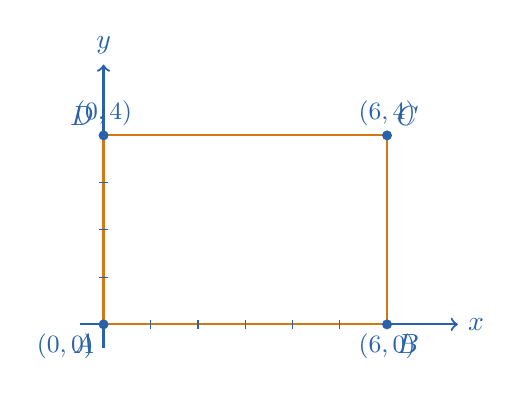
\begin{tikzpicture}[scale=0.6]
  \draw[->, thick, mainblue] (-0.5,0) -- (7.5,0) node[right]{$x$};
  \draw[->, thick, mainblue] (0,-0.5) -- (0,5.5) node[above]{$y$};
  \draw[thick, examorange] (0,0) rectangle (6,4);
  \fill[mainblue] (0,0) circle(3pt) node[below left]{$A$};
  \fill[mainblue] (6,0) circle(3pt) node[below right]{$B$};
  \fill[mainblue] (6,4) circle(3pt) node[above right]{$C$};
  \fill[mainblue] (0,4) circle(3pt) node[above left]{$D$};
  \node[mainblue] at (0,0) [below left]{\small $(0,0)$};
  \node[mainblue] at (6,0) [below]{\small $(6,0)$};
  \node[mainblue] at (6,4) [above]{\small $(6,4)$};
  \node[mainblue] at (0,4) [above]{\small $(0,4)$};
  % 刻度
  \foreach \x in {1,2,3,4,5,6}
    \draw[mainblue] (\x,0.1) -- (\x,-0.1);
  \foreach \y in {1,2,3,4}
    \draw[mainblue] (0.1,\y) -- (-0.1,\y);
\end{tikzpicture}
\end{center}

$A(0, 0)$，\quad $B(6, 0)$，\quad $C(6, 4)$，\quad $D(0, 4)$。

\begin{tipbox}[方法总结]
建立坐标系解题的步骤：
\begin{enumerate}[leftmargin=1.5em]
  \item 选取合适的点作为原点（通常选顶点或特殊点）。
  \item 确定坐标轴方向（通常沿边或对称轴方向）。
  \item 根据已知边长，逐个求出各点坐标。
\end{enumerate}
\end{tipbox}

\bigskip

\begin{examplebox}[【例题7】综合题——已知坐标关系求字母的值]
已知点 $P(a + 2,\ 3a - 6)$ 在 $y$ 轴上，求点 $P$ 的坐标。
\end{examplebox}

\textbf{解：}

点 $P$ 在 $y$ 轴上，说明横坐标为 $0$，即：
$$a + 2 = 0 \Rightarrow a = -2$$

代入纵坐标：$3 \times (-2) - 6 = -6 - 6 = -12$。

所以 $P$ 的坐标为 $\boxed{(0, -12)}$。

% ==============================================================
% 第三部分：应用题
% ==============================================================
\section*{\textcolor{apppurple}{三、应用题}}

\begin{appbox}[【应用1】用坐标表示学校地图]
下图是某学校的平面示意图（每个方格的边长代表 $50$ 米）。以校门为原点，正东方向为 $x$ 轴正方向，正北方向为 $y$ 轴正方向建立坐标系。

\begin{center}
\begin{tikzpicture}[scale=0.55]
  \draw[->, thick, mainblue] (-1,0) -- (7,0) node[right]{\small $x$（东）};
  \draw[->, thick, mainblue] (0,-1) -- (0,6) node[above]{\small $y$（北）};
  \node[mainblue] at (0,0) [below left]{\small 校门};
  % 方格
  \foreach \x in {0,...,6}
    \foreach \y in {0,...,5}
      \draw[gray, very thin] (\x-0.5,\y-0.5) rectangle (\x+0.5,\y+0.5);
  % 标记建筑
  \fill[examorange] (1,2) circle(3pt) node[right]{\small 教学楼};
  \fill[tipgreen] (4,3) circle(3pt) node[right]{\small 图书馆};
  \fill[apppurple] (3,1) circle(3pt) node[right]{\small 操场};
  \fill[warnred] (5,4) circle(3pt) node[right]{\small 食堂};
\end{tikzpicture}
\end{center}

\begin{enumerate}[label=(\arabic*)]
  \item 写出教学楼、图书馆、操场、食堂的坐标。
  \item 如果教学楼要举办活动，需要在它正北方向 $100$ 米处挂横幅，横幅挂在哪？
\end{enumerate}
\end{appbox}

\textbf{解：}

\begin{enumerate}[label=(\arabic*)]
  \item 教学楼 $(1, 2)$，图书馆 $(4, 3)$，操场 $(3, 1)$，食堂 $(5, 4)$。每个单位代表 $50$ 米。
  \item 教学楼在 $(1, 2)$，正北方向 $100$ 米即向北 $2$ 个单位。横幅挂在 $(1, 4)$ 的位置。
\end{enumerate}

\bigskip

\begin{appbox}[【应用2】用坐标和对称解决实际问题]
已知正方形 $ABCD$ 的三个顶点为 $A(0, 0)$，$B(4, 0)$，$C(4, 4)$。
\begin{enumerate}[label=(\arabic*)]
  \item 求第四个顶点 $D$ 的坐标。
  \item 求正方形的中心（对角线交点）$O$ 的坐标。
  \item 正方形 $ABCD$ 关于 $x$ 轴对称的正方形为 $A'B'C'D'$，求 $A'$、$B'$、$C'$、$D'$ 的坐标。
\end{enumerate}
\end{appbox}

\textbf{解：}

\begin{enumerate}[label=(\arabic*)]
  \item 由 $A(0,0)$、$B(4,0)$、$C(4,4)$ 可知 $AB$ 沿 $x$ 轴方向长 $4$，$BC$ 沿 $y$ 轴方向长 $4$。$D$ 与 $A$ 同横坐标、与 $C$ 同纵坐标，故 $D(0, 4)$。

  \item 中心 $O$ 为对角线 $AC$ 的中点：
        $$O = \left(\dfrac{0+4}{2},\ \dfrac{0+4}{2}\right) = (2, 2)$$

  \item 关于 $x$ 轴对称，横坐标不变，纵坐标变号：
        $$A'(0, 0),\quad B'(4, 0),\quad C'(4, -4),\quad D'(0, -4)$$

        \begin{center}
        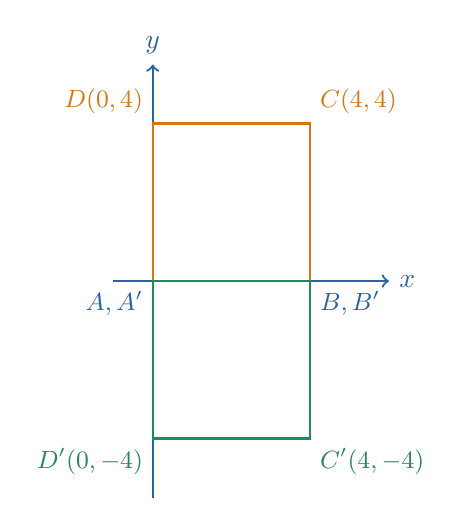
\begin{tikzpicture}[scale=0.5]
          \draw[->, thick, mainblue] (-1,0) -- (6,0) node[right]{$x$};
          \draw[->, thick, mainblue] (0,-5.5) -- (0,5.5) node[above]{$y$};
          \draw[thick, examorange] (0,0) rectangle (4,4);
          \draw[thick, tipgreen] (0,0) rectangle (4,-4);
          \node[examorange, font=\small] at (4,4) [above right]{$C(4,4)$};
          \node[examorange, font=\small] at (0,4) [above left]{$D(0,4)$};
          \node[mainblue, font=\small] at (0,0) [below left]{$A,A'$};
          \node[mainblue, font=\small] at (4,0) [below right]{$B,B'$};
          \node[tipgreen, font=\small] at (4,-4) [below right]{$C'(4,-4)$};
          \node[tipgreen, font=\small] at (0,-4) [below left]{$D'(0,-4)$};
        \end{tikzpicture}
        \end{center}
\end{enumerate}

\bigskip

\begin{appbox}[【应用3】机器人走格子]
一个机器人在平面直角坐标系中从原点 $O(0, 0)$ 出发，按以下规则运动：先向右走 $1$ 步到 $(1, 0)$，再向上走 $1$ 步到 $(1, 1)$，再向左走 $2$ 步到 $(-1, 1)$，再向上走 $2$ 步到 $(-1, 3)$，再向右走 $3$ 步到 $(2, 3)$\ldots 按此规律继续走。请问：走完第 $10$ 步时，机器人的坐标是什么？
\end{appbox}

\textbf{解：}

观察运动规律，每两步为一组：

\begin{center}
\renewcommand{\arraystretch}{1.3}
\begin{tabular}{|c|c|c|c|}
\hline
\textbf{组} & \textbf{步数} & \textbf{方向} & \textbf{到达坐标} \\
\hline
第1组 & 1--2 & 右1，上1 & $(1, 1)$ \\
\hline
第2组 & 3--4 & 左2，上2 & $(-1, 3)$ \\
\hline
第3组 & 5--6 & 右3，上3 & $(2, 6)$ \\
\hline
第4组 & 7--8 & 左4，上4 & $(-2, 10)$ \\
\hline
第5组 & 9--10 & 右5，上5 & $(3, 15)$ \\
\hline
\end{tabular}
\end{center}

第10步结束时，机器人的坐标为 $\boxed{(3, 15)}$。

% ==============================================================
% 第四部分：课堂练习
% ==============================================================
\section*{\textcolor{tipgreen}{四、课堂练习}}

\begin{enumerate}[label=\textbf{\arabic*.}, leftmargin=2em]
  \item 填空：
  \begin{enumerate}[label=(\arabic*)]
    \item 点 $(2, -5)$ 在第\blank{1cm}象限。
    \item 点 $(0, 7)$ 在\blank{1cm}轴上。
    \item 点 $(-3, -4)$ 到 $x$ 轴的距离为\blank{1cm}，到 $y$ 轴的距离为\blank{1cm}。
  \end{enumerate}

  \item 点 $P(-2, 3)$ 关于 $x$ 轴对称的点的坐标为\blank{1.5cm}；关于 $y$ 轴对称的点的坐标为\blank{1.5cm}；关于原点对称的点的坐标为\blank{1.5cm}。

  \item 将点 $A(3, -1)$ 向左平移 $5$ 个单位，再向上平移 $3$ 个单位，所得点的坐标为\blank{1.5cm}。

  \item 已知点 $M(2a - 1,\ a + 3)$ 在第二象限，求 $a$ 的取值范围。

  \item 已知点 $N(x, y)$ 满足 $|x - 2| + |y + 3| = 0$，求点 $N$ 的坐标。

  \item 在平面直角坐标系中，已知 $A(1, 0)$，$B(5, 0)$，点 $C$ 在 $y$ 轴上，且 $\triangle ABC$ 的面积为 $8$，求点 $C$ 的坐标。

  \item 已知点 $P(a, b)$ 到 $x$ 轴的距离等于到 $y$ 轴的距离，写出所有满足条件的点 $P$ 的坐标特征。

  \item 一个正方形的三个顶点分别为 $A(0, 0)$，$B(4, 0)$，$C(4, 4)$，求第四个顶点 $D$ 的坐标。
\end{enumerate}

\bigskip

\begin{knowledgebox}[参考答案]
\textbf{1.}
\begin{enumerate}[label=(\arabic*)]
  \item 四 \quad (2) $y$ \quad (3) $4$；$3$
\end{enumerate}

\textbf{2.}\quad $(-2, -3)$；\quad $(2, 3)$；\quad $(2, -3)$

\medskip
\textbf{3.}\quad $(-2, 2)$

\medskip
\textbf{4.} 点 $M$ 在第二象限，则 $2a - 1 < 0$ 且 $a + 3 > 0$。解得 $a < \dfrac{1}{2}$ 且 $a > -3$，所以 $\boxed{-3 < a < \dfrac{1}{2}}$。

\medskip
\textbf{5.} $|x - 2| \geqslant 0$，$|y + 3| \geqslant 0$，两者之和为 $0$，则 $x - 2 = 0$，$y + 3 = 0$，故 $x = 2$，$y = -3$，$N(2, -3)$。

\medskip
\textbf{6.} $AB = 5 - 1 = 4$。设 $C(0, c)$，$\triangle ABC$ 的面积 $= \dfrac{1}{2} \times 4 \times |c| = 8$，故 $|c| = 4$，$c = \pm 4$。所以 $C(0, 4)$ 或 $C(0, -4)$。

\medskip
\textbf{7.} $|a| = |b|$，即 $a = b$ 或 $a = -b$。点 $P$ 在直线 $y = x$ 或直线 $y = -x$ 上。

\medskip
\textbf{8.} 由 $A(0,0)$、$B(4,0)$、$C(4,4)$ 可知正方形为 $ABCD$，$D(0, 4)$。
\end{knowledgebox}

\vfill
\begin{center}
\small\textcolor{gray}{本讲义仅供教学参考，例题可根据学生水平调整难度。}
\end{center}

\end{document}
